\section{Introduction}

In this article we outline the theoretical background for some of
the empirical studies performed within the frame of our respective
artistic PhD projects at the Malm� Academy of Music, Lund University.
The purpose of the studies performed and hence, the
requirements of the methods we use to perform them and study their
outcome, is to explore the inter-relations between performer and
composer. Specifically we study the musical work in
the Western art music tradition, prior to its ultimate
notation and prior to its performance. Though many of the
ideas presented below may apply to other genres this article is mainly
concerned with music for solo instrument and live electronics.

Trevor Wishart introduces the idea that the development of notation
has, among many other things, resulted in a division of the musician
into `composer' and `performer' \citep{wis96}. This split calls for an
extended discussion of what composer and performer provide to the
creative process. Our ambition is to approach this issue by studying
the low-level processes leading up to a version of the musical work.
We find that by using the concept of `agents' we bypass the otherwise
problematic values traditionally assigned to the two labours. The
musical work as an open concept, such as it is developed by Lydia
Goehr in her book \emph{The Imaginary Museum of Musical Works} (1992),
is also central to the reasoning in this paper as well as her claim,
that the work concept has had a regulative function only at certain
times in the history of Western art music. In contemporary music this
regulative function can be found to be pertinent in one composer's
work and extraneous in another's.

\section{The Ontology of the Musical Work}\label{sec:ontology}

A musical work, in the cultural context of the Western art music
tradition, and especially since the romantic era up to the present
day, is commonly regarded as the result of a process in two distinct
phases; one constructive and one reproductive. The composer produces a
score, which in turn is handed over to a performer who makes an
interpretation of the notation and reproduces it as specified in the
score. The score constitutes the primary source of information (see
Figure \ref{cons-rep}).

 \begin{figure}[!htb]
 \begin{center}
  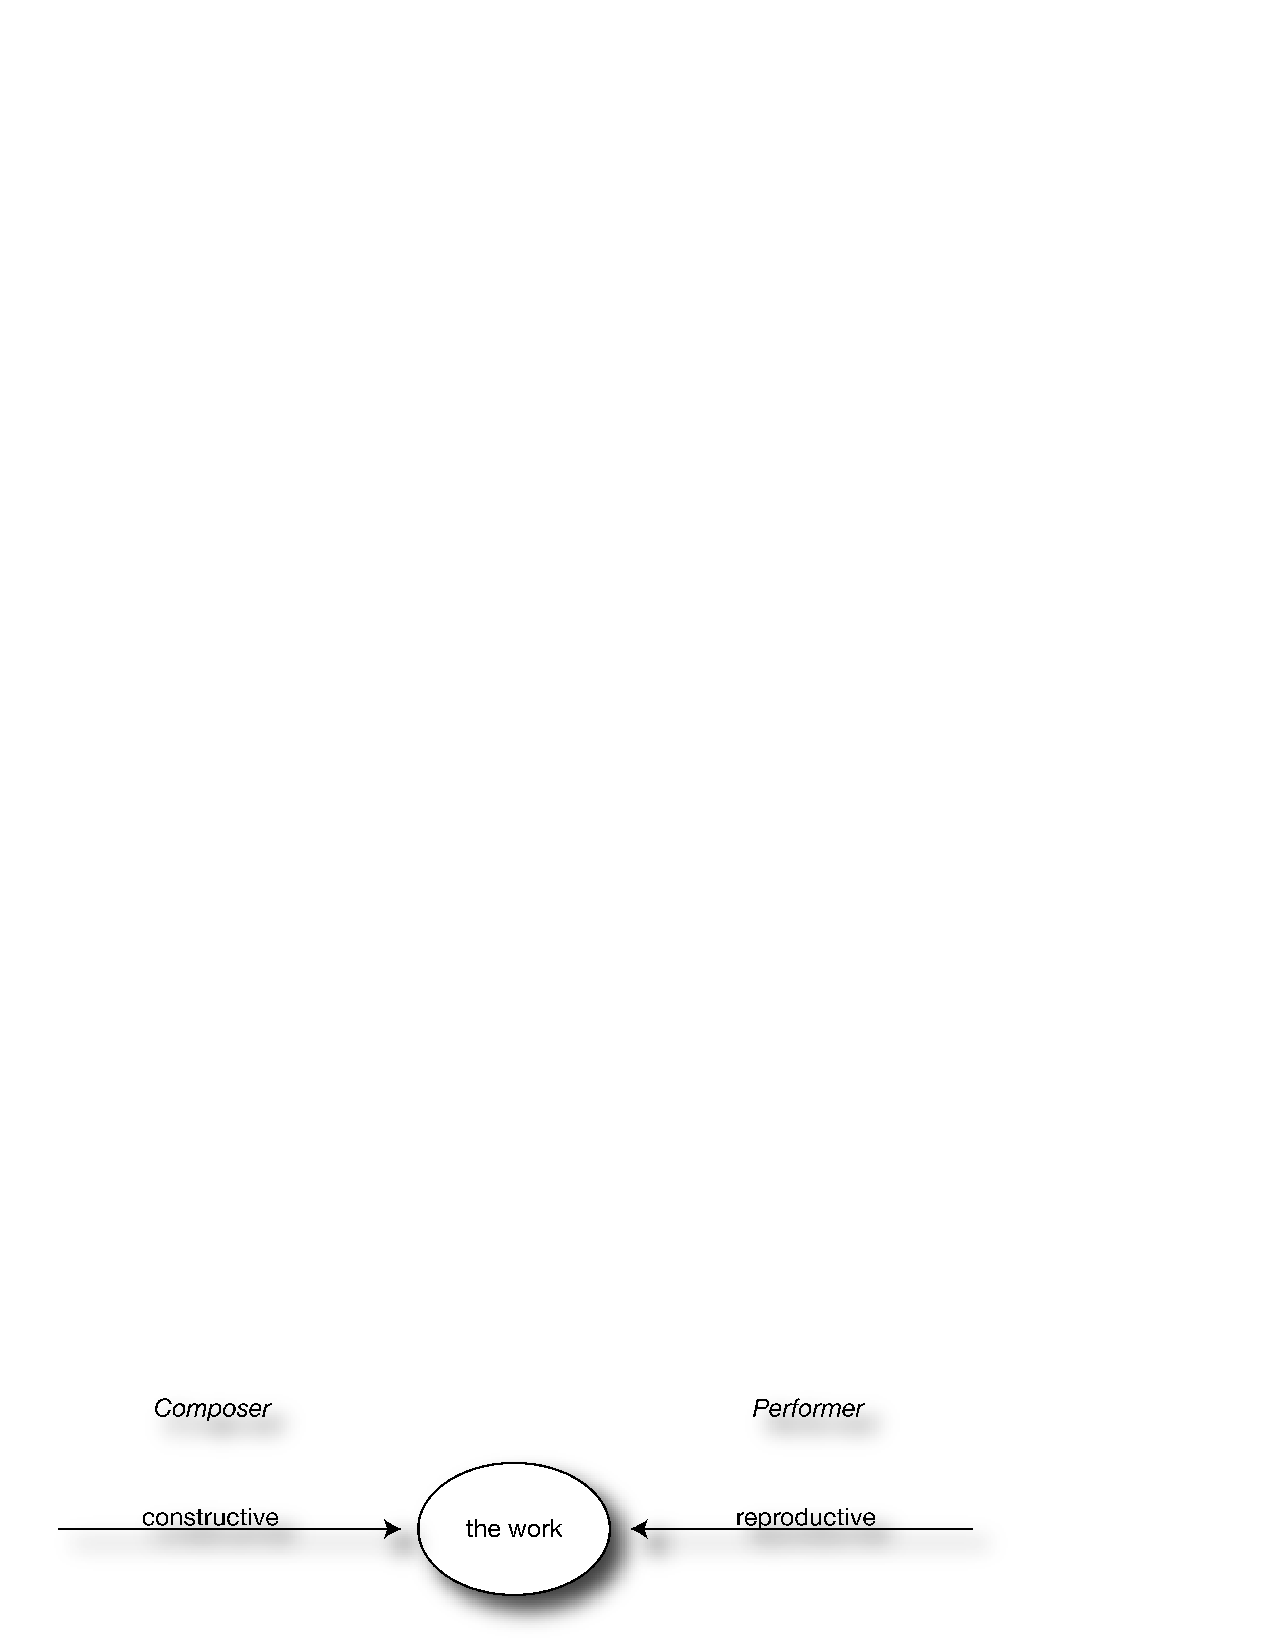
\includegraphics[width=0.8\columnwidth]{img/cons-rep2}
  \caption{Within the Western art music tradition the score is commonly
  regarded as the primary source of information.}
  \label{cons-rep}
 \end{center}
 \end{figure}

 In Paul Ric{\oe}ur's hermeneutic philosophy, the traditional view of
 the author as a one-way sender of a message is disputed. Ric{\oe}ur
 finds that the author is disengaged from the work by the act of
 writing \citep{ric91}. When writing takes the place of dialogue, the
 immediate face-to-face communication is replaced by inscription and
 the semantic autonomy of the text. The disconnection between the
 author's intention and the meaning of the text is a key issue in
 Ric{\oe}ur's theory. The inscription of a discourse in writing brings
 the semantic autonomy of language into play.

\begin{quote}
  The text is the very place where the author appears. But does the
  author appear otherwise than as first reader? The distancing of the
  text from its author is already a phenomenon of the first reading
  that, in one move, poses the whole series of problems that we are
  now going to confront concerning the relations between explanation
  and interpretation. These relations arise at the time of reading.
  \citep[p. 109-10]{ric91}
\end{quote}

Suppose that we undertake the hypothetical experiment of applying this
theory on the literary text to musical production: are there any
analogies between Ric{\oe}ur's account and musical practice? Imagine
music-making, as it takes place independently of musical notation, as
compared to the kind of dialogue that the inscription of text
replaces. Improvisation involves making variations on known patterns,
and when this is successful, truly innovative music comes out. Imagine
a composer writing music: Isn't it necessary for him to interact with
the musical `language', or context, in which he is working, in a
similar way as is necessary for the improviser? Analogically speaking,
the moment that the composer starts making the notation, the
'dialogue' is replaced by the semantic autonomy of the text-based
musical context, with its own structural possibilities and
limitations. The composer is detached from the music in the act of
notating it. In the case of a written text, the intention of the
author is not equal to the meaning of the text. The author is present
in the text, but only as a first reader. Similarly, this suggests that
the construction of a score-based work consists of dialectic interplay
between creation and interpretation, in which the composer - even
during the act of writing - has to approach the notation by means of
interpretation.

By this reflection on the artistic process, and in the light of
Ric{\oe}ur's philosophy, the view of the composer representing the
productive phase, and the performer the reproductive, is questioned.
We arrive at a modification of the traditional scheme of
construction/reproduction, instead involving construction, but also
interpretation in the composer's creative process.

\begin{figure}[!htb]
  \begin{center}
    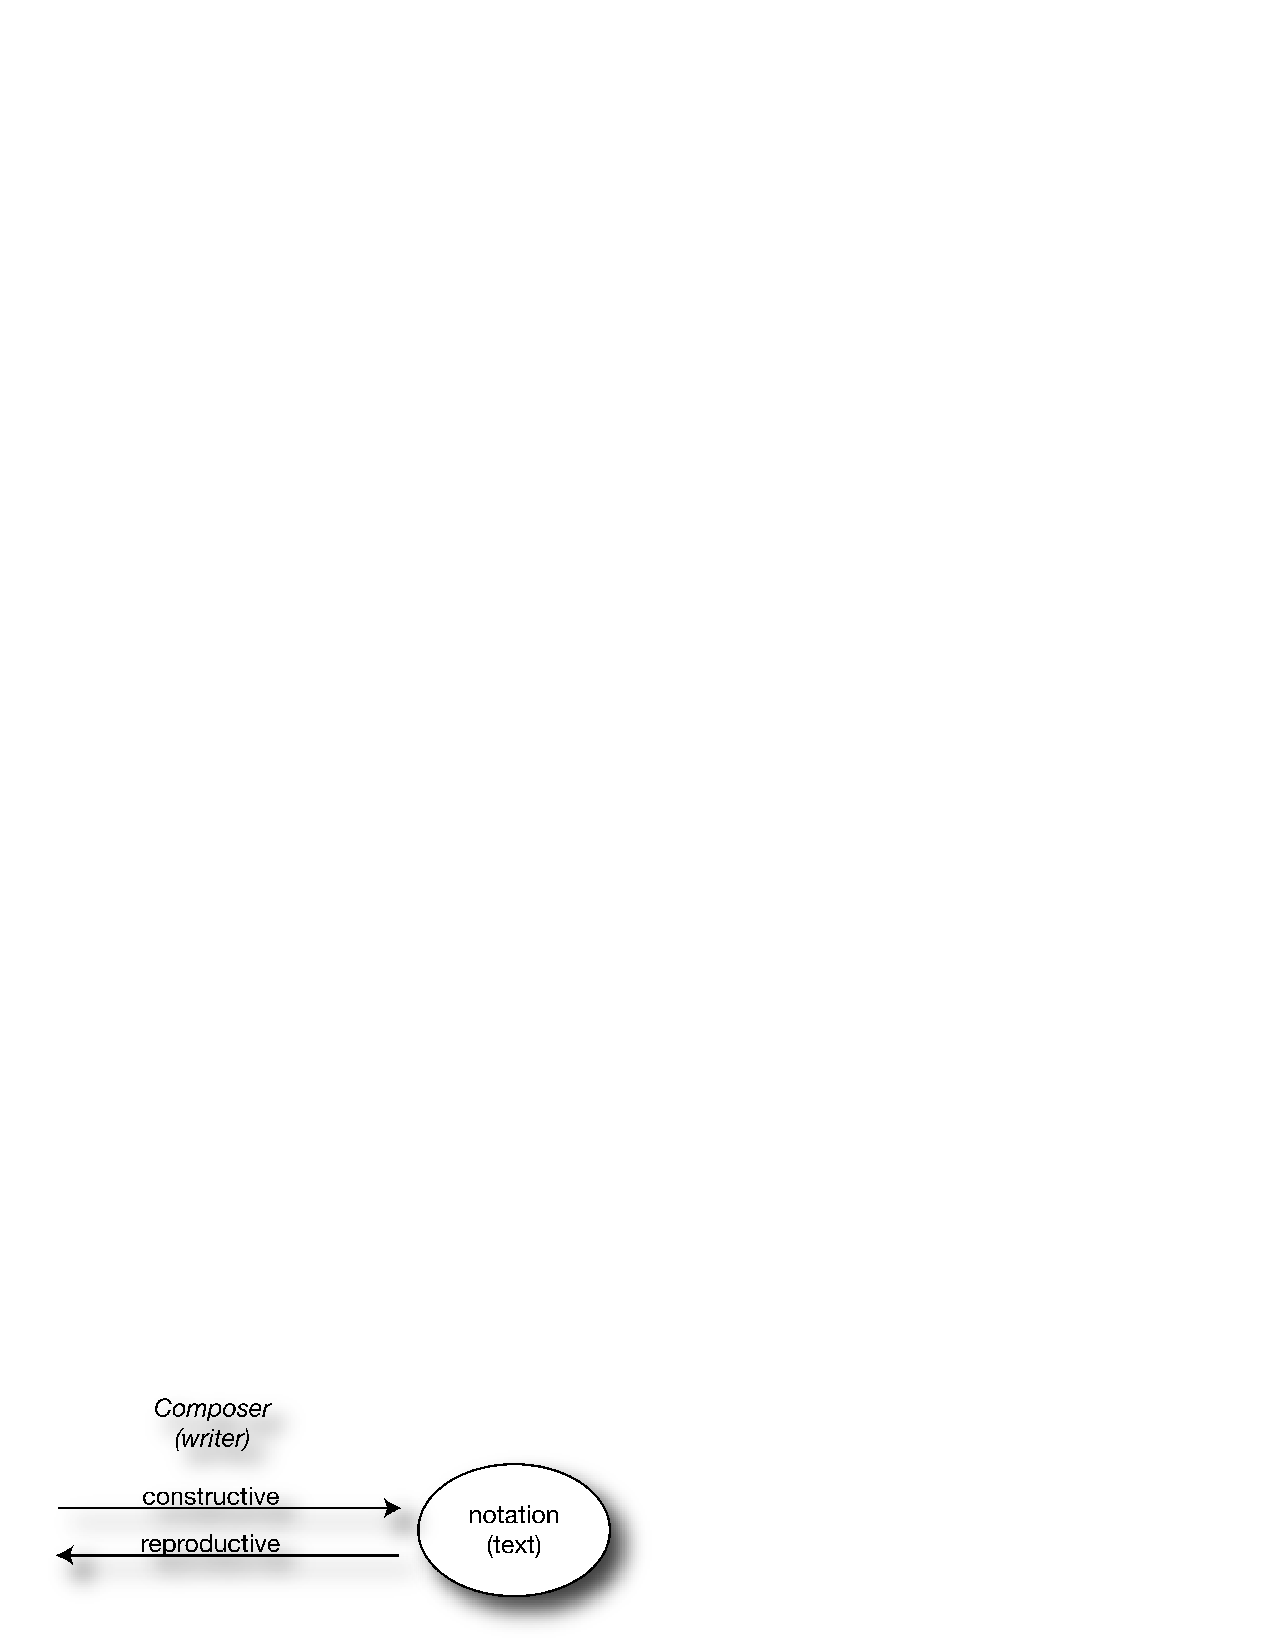
\includegraphics[width=0.8\columnwidth]{img/cons-rep-ric2}
    \caption{In the light of Ric{\oe}ur we arrive at a modified scheme
      involving construction as well as interpretation in the composer's creative
      process.}
    \label{cons-rep2}
  \end{center}
\end{figure}

Another aspect of the composer's practice is highlighted by
Horacio Vaggione \citep{vaggione01}. The composer always has to
approach the process of producing a piece of music as a listener,
either in the form of inner listening while writing an instrumental
score or the concrete listening in the production of a pure electronic
piece. This is described by Vaggione as an action/perception feedback
loop, reminiscent of the notation/interpretation process suggested by
the thinking of Ric{\oe}ur. But there is a fundamental difference
between the two accounts: what Vaggione provides is a theoretical
reflection on the kind of thinking that is not based on language, but on
action and perception.

\begin{quote}
 In order to produce music an act of hearing is necessary, whether it
 be the `inner hearing' (the silent writing situation) of pure
 instrumental music composition, or the `concrete hearing' of
 electroacoustic music composition. These situations involve variants
 (there are many others) of an `action/perception feedback loop' which
 can be defined as an instance of validation proper to musical
 processes. \citep{vaggione01}
\end{quote}
Without any further specification, Vaggione hints at the many other
 variants of this class of feedback loops at play in the production of
 musical content. It is important to bear in mind that `thinking' in
 modes of action does not require a `transcription' into language.
 What Vaggione reminds us is that `thinking through hearing' and
 `thinking through performing' are essential modes of interpretation.
 These involve the physical interaction between a performer and his or
 her instrument as well as the inner listening of the composer; both
 of which do not require verbal translation. This kind of
 interpretation is what we would call `thinking through
 practice'.\footnote{One important source for the notion of `thinking
   through practice' is the thinking of Art historian and curator
   Sarat Maharaj. His introductory paper for the \emph{Knowledge Lab}
   at the \emph{Haus der Kulturen der Welt in Berlin} 2005 (in which both
   authors participated) was entitled `Thinking Through Performance'
   and discussed how various modes of `thinking through' could
   function as a methodology for the creation of new knowledge in the
   arts. We believe that the way we use the term in the present paper
   makes a slightly different use of the notion of `thinking through':
   in the \emph{Knowledge Lab}, `thinking through' referred to a mode of
   studying artistic practice, whereas we use the notion to describe
   processes within artistic practice itself. One could argue that
   our study gives further confirmation to the methodology suggested
   by Maharaj for the \emph{Knowledge Lab}.}

Our conclusion is that the
 use of notation and the subsequent musical practice that has followed
 from it, does not unambiguously divide composer and performer into
 one `auteur' (producing the work) and one interpreter (reproducing
 it). Interpretation is a part of both creative acts and the
 practices of both agents overlap in many ways.

\begin{figure}[!htb]
  \begin{center}
    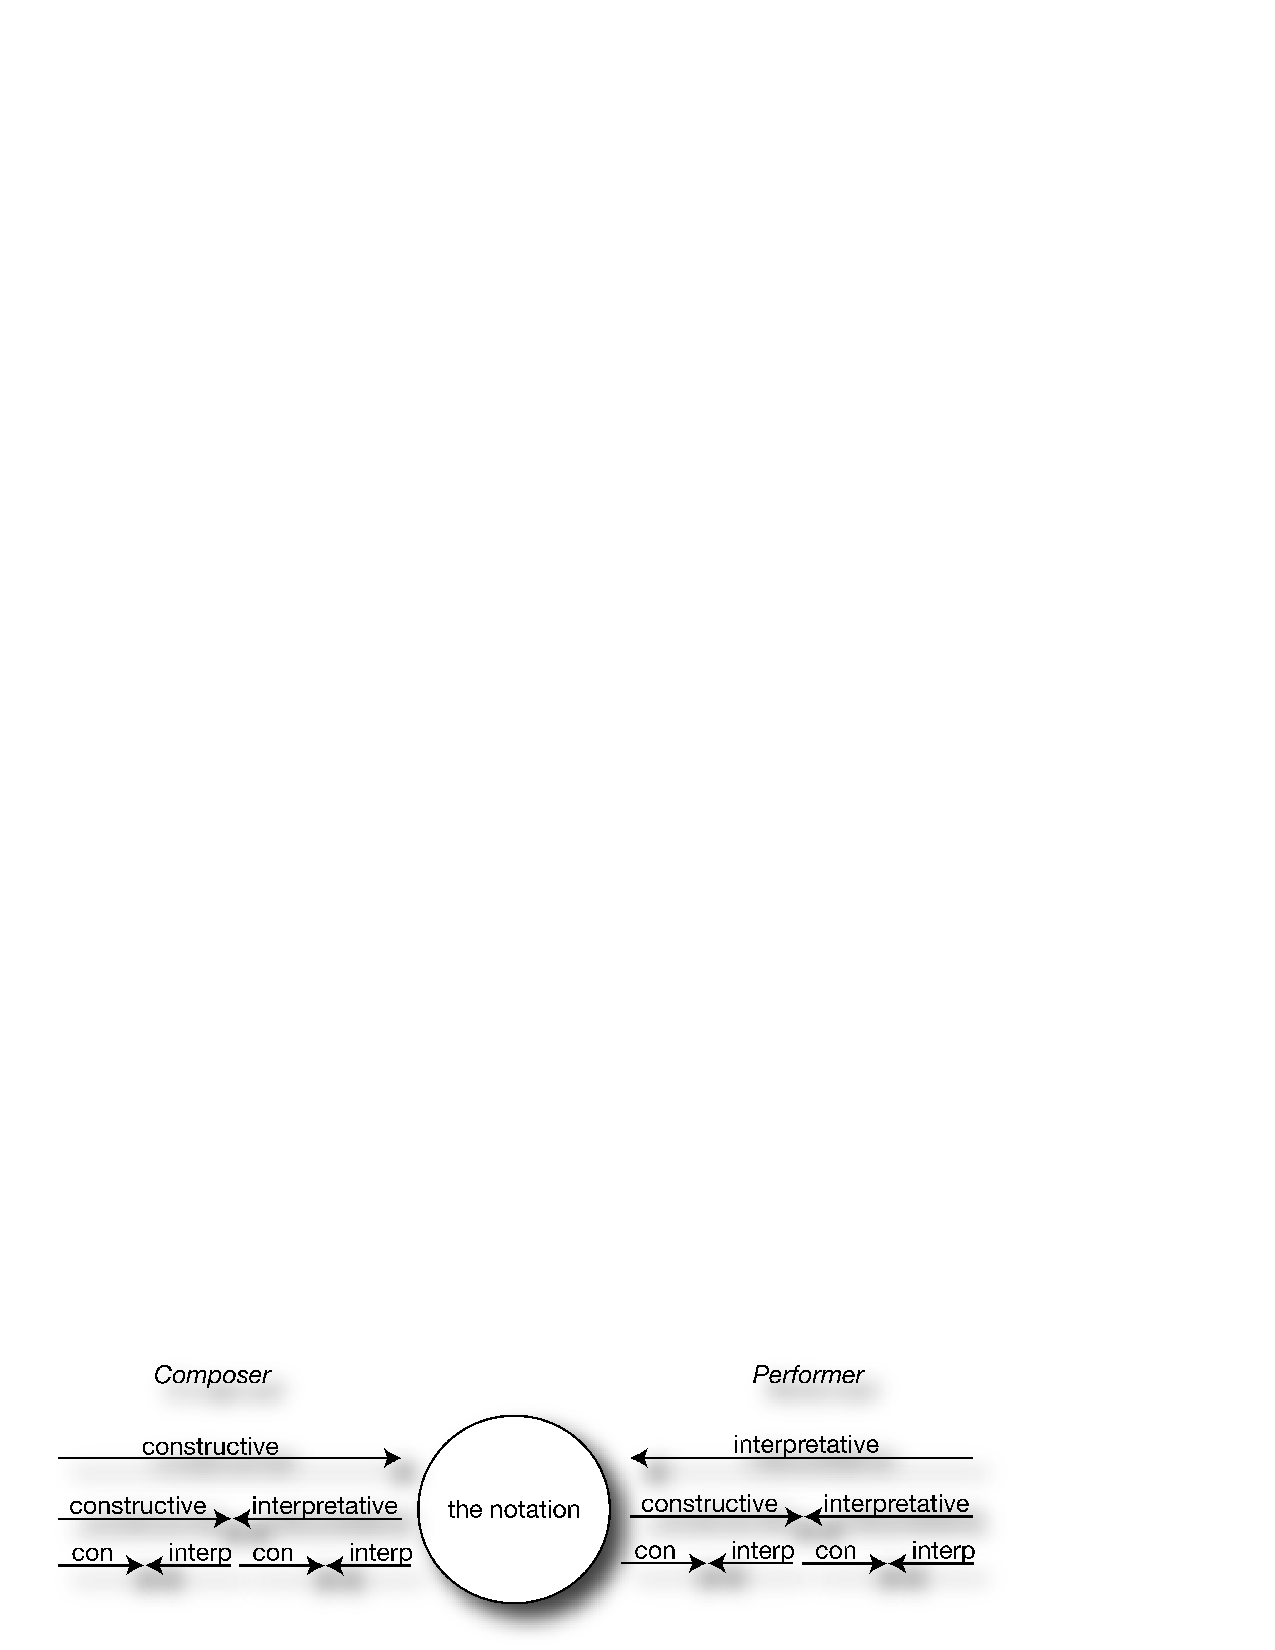
\includegraphics[width=0.8\columnwidth]{img/cons-rep-rep-cons2}
    \caption{Our schematic model of the interaction between
      constructive and interpretative phases in performance and
      composition.}
    \label{cons-rep3}
  \end{center}
\end{figure}

\subsection{Musical Interpretation and performance} \label{subsec:musical_interpretation}

Since the 19th century, performances of score-based works have
commonly been referred to as interpretations. If we regard
performances as interpretations, are they interpretations of the
notation or of a wider entity? This is in essence a matter of the
ontology of the musical work: Is the work equivalent to the score or
is there more to the identity of the work than notation? According to
Theodor Adorno, the ``musical score is never identical with the work;
devotion to the text means the constant effort to grasp that which it
hides [...]'' \citep[p. 144]{adorno81}. A crucial fact about musical works
is their historicity. Firstly in the sense that the material that is
available to the composer is historically and culturally mediated and
thus pre-formed within the cultural context in which he is working.
Secondly, meaning in music, and in Adorno's view this also equals the
musical work itself, is achieved in the tension between the received
formal norms and the `second reflection' or re-contextualisation in
the compositional process by the creative `Subject' \citep{pad91}. The
work is not equivalent to the score but is a cultural construct that
materialises in its relation to its cultural context.

Paul Ric{\oe}ur introduces the concept of the `world of the text' as
something other than the intention of the author. The meaning of the
text is projected in front of the text, and is not to be found in
authorial intent `behind' the text, as in romantic hermeneutic
philosophy. What is unfolded by the passing from explanation to
understanding is the thing of the text, or the kind of world that the
text unfolds before the text.

\begin{quotation}
Reading is no longer simply listening. It is governed by codes
comparable to the grammatical code that guides the understanding of
sentences. In the case of the narrative, these codes are precisely the
ones that a structural analysis brings to light under the title of
narrative codes.

It cannot, therefore, be said that the passage by way of explanation
destroys intersubjective understanding. This mediation is required by
discourse itself. I am expressly using the term discourse and not
simply speech, the fugitive manifestation of language. For it is
discourse that calls for this ever more complicated process of
exteriorization with regard to itself, a process that begins with the
gap between saying and the said, continues through the inscription in
letters, and is completed in the complex codifications of works of
discourse, the narrative among others. Exteriorization in material
marks and inscription in the codes of discourse make not only possible
but necessary the mediation of understanding by explanation, of which
structural analysis constitutes the most remarkable
realization. \citep[p. 130]{ric91}
\end{quotation}

Not only is the author detached from the work by the act of writing.
For a reader to enter into the world of the text, a similar process of
detachment and analytical interpretation is needed. But writing music
is an activity distinct from writing a literary text. A score, to a
higher degree than is a text, is a tacit agreement with a present or
implied performer - we cannot simply equal a verbal text to a score and
a performer to a reader of this text. But there seems to be an
immanent call for analysis and interpretation in the construction of
musical meaning. Musical meaning may be found through a movement from
explanation through analysis to understanding.

\begin{quotation}
The performance of a piece of music is (...) the actualisation of an
analytic act - even though such analysis may have been intuitive and
unsystematic. For what a performer does is to make the relationships
and patterns potential in the composer's score clear to the mind and
ear of the experienced listener. \citep[p. 29]{meyer73}
\end{quotation}

From a general point of view, interpretation in the context of the
arts can be understood as assigning meaning to works. To what
extent can we claim that performances do this? Turning to definitions,
we will now attempt to trace the difference between critical
interpretation and what we tend to call performance interpretation.
\begin{quotation}
Being an interpretation of is a relation between a thought or an
utterance on the one hand and an object of interpretation on the
other. In the case of art (...) an utterance about a work is an
interpretation of the work, only if it says something about the
meaning of a work, about a meaning it could have or was intended to
have, or about the work's significance. \citep[p. 82]{stecker}
\end{quotation}
Stecker's definition of interpretation raises some important
questions: What musical actions do we regard as interpretation, and in
what sense do they assign meaning to the work? 

Are the performer's shaping of phrases, relative level of dynamics and
accents etc. really to be regarded as an interpretation of the piece,
assigning meaning to the music? Markings by the composer of dynamics,
accentuation, phrasing etc are often regarded as `interpretative'.
This mode of speaking implies that markings of this kind represent the
author's interpretation of the meaning of the work. But this seems
implausible to us. Isn't it more likely that the reason we tend to
regard these markings as interpretational is that they represent a
category of musical organisation that often has been left to the
performer's discretion? According to our understanding of the musical
event all parameters belong to the musical fact.

In the preparatory stages the performer has to make decisions of a
kind that do not clearly differ from that of critical interpretation
\citep[38-9]{levinson}. In order to take a position in cases where a
score is incomplete, inconsistent or exists in different versions, a
critical interpretation of the score is necessary. This could imply
that the difference between critical and performative interpretations
is of a floating and unclear kind. On the contrary Levinson argues
that they are logically distinct activities.

\begin{quotation}
...a critical interpretation typically aims to explain (or elucidate)
a work's meaning or structure - "what is going on in it", in a common
phrase - whereas a performative interpretation can at most highlight
(or effectively display) that meaning or structure. A performative
interpretation, if successful, may enable one to conceive of a work
differently in the critical sense - as the performer conceived it in
arriving at the performative interpretation - but only a critical
interpretation indicates or details such a conception. \citep[p. 38-9]{levinson}
\end{quotation}
In other words, there are many ways in which a performance fails to
fulfil the criteria for a critical interpretation. In critical
interpretation we do not have this peculiar amalgamation of `object of
interpretation' and the `interpretation' itself. This crucial
difference between performance and critical interpretation is also
acknowledged by Robert Stecker:
\begin{quotation}
If performances and critical interpretations are both representations
of works, they are so in quite different senses. If we ignore these
differences, we can easily be misled to make invalid inferences.
Performances are necessarily constructive; that is, they necessarily
add features that the work leaves vague or undetermined. \citep[p. 80]{stecker}
\end{quotation}
But not only in cases in which the notation is in some respect unclear
or vague is there a call for constructive elements in performance.
Construction is really at the heart of the matter. The relation
between a performance interpretation and the work is not the relation
between an external receiver and an artwork but the relation between
different forces at play in the construction of the work itself. The
use of notation presumes a common understanding of performance
practice of composer and interpreter. This fundamental agreement
between a composer and an imagined or present performer is part and
parcel of every musical notation. As we have seen in the thinking of
Adorno and furthered into the model of `the world of the text', a true
instance of a work must be based on an interpretation that goes beyond
the mere text of the score. Assigning meaning to a musical work is
achieved by way of a critical reading of the work (and not only the
score). Musical meaning is constructed in the relation between the
musical structures themselves and the musico-historical context - its
tradition - and the friction between this context and the work.

In the preservatory culture that Classical Music is today, we tend to
speak of works as ideal objects that are `interpreted' in performances
that can be evaluated in comparison with this ideal entity. However,
we find that musical interpretation is better understood as an
analytical and hermeneutic tool that is a part of the agencies of the
performer as well as the composer. Performances are not separate from
the work but always a part of it - a successful performance is an
embodiment of the work\footnote{This is not to say that performances
  cannot be more or less true to the instructions in the score, or to the
  tradition, and that the performance itself should not be accessible
  for critical consideration.}:
\begin{quotation}
Every performance is an event, but not one that would in any way be
separate from the work - the work itself is what `takes place' in the
performative event.\citep{gad60}
\end{quotation}
We would like to propose the fairly radical idea of dropping the term
performance interpretation. Preceding performance is an act of
interpretation, either by means of analytical thinking (critical
interpretation) or through an embodied mode of `thinking through
practice'. However, it is important to bear in mind that, just as
Gadamer reminds us, a performance is not to be understood as an
interpretation of a work, but as its final constructive phase.

\section{Musical semiology}\label{sec:musical_semiology}

In his 1989 article `Reflections on the development of semiology of
music' Jean-Jacques Nattiez offers an excellent review of the history
of musical semiology. In it he gives an historic perspective on the
fundamental issue of the nature of musical signification. Nattiez
distinguishes between intrinsic and extrinsic significations within
musical semantics, finding the theory of the former to be to a large
extent founded on the work of Nicolas Ruwet and the notion of music as
a language that signifies itself \citep[p. 30]{nat89}. Jean Molino
summarizes Susanne Langer's idea of music as the `unconsummated
symbol' and captures the essence of the problem: ``On the one hand,
the unchallengeable presence of evocation; on the other, the
impossibility of exploiting it'' \citep[p. 126-7]{molino}. Molino aims
at a theory in which music is understood as networked communication or
exchanges between individuals. As we will discuss more thoroughly in
the next section, the sender and receiver do not have to come to the
same understanding of the message, or the `trace' as Molino would call
it, hence there is no need for a understanding of the `code' which is
significant to the semiosis favored by Umberto Eco. Eco points to the
problems with connecting the investigation of a sign with the object
to which it refers. It is impossible to attribute logical statements
such as `true' or `false' to the semiological investigation of music
and for Eco these are pre- or postsemiotic problems; ``The signs are
of interest to semiotics as social powers'' and further ``Any attempt
to establish the referent of a sign will force us to define this
referent with the terminology of an abstract entity.'' This is what
Eco calls the ``cultural convention''. \citep[p. 61-6]{eco71}

Defining a cultural context as the referent resolves some issues in
the analysis of performed music as a social fact. The listener or
concert-goer can be defined as belonging to a cultural entity with
predetermined understandings of the context of the performance, but
also of the cultural markers within the music. This cultural entity
may then be used as a code to decipher the message (the music as a
symbolic system). However, in our study we are looking at a not yet
existing work - a work in progress - and we are not primarily
interested in the symbolic understanding of \emph{music} as it is
materialized in the physical world. Our focus is geared towards the
understanding of the \emph{actions} that lead to production of musical
content. Following Eco's model we might try to approach this symbolic
system in relation to a common context, or subculture created by the
agents involved in it. Both composer and performer are working within
the frame of their own cultural contexts which defines their
respective understandings of the evolving work. The subculture is a
result of interaction, and negotiation ('\emph{What is it we are
 developing?}', '\emph{How are we talking about it?}', etc.), between
the two agents and their inherent cultural contexts. Their mutual
expectations and their understanding or imagination of the work in
progress is of importance when they attempt at co-ordinating their
actions, for instance towards a definition of the performance
instructions. The musical work becomes the sign or the message, the
agents the signifiers and the subculture the signified. Where,
traditionally, we may tend to regard the composer/performer relation
as a hierarchic structure in which the role, even the purpose, of the
performer is to fulfill the composer's intentions (whether he is dead
or alive), this mode of analysis allows us to look at the two agents
as part of a larger system that may also contain many other agents.

But to fully understand the dynamics of the context, or subculture as
we call it, we also need the tools to move to a lower level of
analysis. The tripartite model suggested by Molino for analysis of
music, though certain aspects of it remains problematic, appears to be
a flexible method for our study at this stage.

\subsection{The three dimensions} \label{subsec:threedim} Molino
reminds us that the hypothesis that there is a ``single, well-defined
item of information to be transmitted, all the rest being simply
noise'' is ``dangerously inaccurate and misleading as soon as we move
from the artificial communication of information to a concrete act of
human communication as a total social fact.'' \citep{molino} Music,
according to him, is a product and not a transmission. The Duchampian
notion of a work of art is very similar; as two poles with the artist
on the one side and the viewer on the other - the intention of the
artist holds no significance to the work's interpretation. Molino
further refers to Paul Val\'{e}ry, to point out that ``there is no
guarantee of a direct correspondence between the effect produced by a
work of art and the intentions of its creator''. The distinction
between what was later coined as the `poietic' and 'esthesic'
dimensions in the symbolic phenomenon was first suggested by
Val\'{e}ry in his inaugural lecture for the Coll\'{e}ge de France in
1945.

The ambition of musical semiology has been to provide tools for an
analytic understanding of the total symbolic fact of the musical work
\citep[p. 34]{nattiez}. Molino argues for a three level symbolic
analysis; ``the poietic, the esthesic and the `neutral' analysis of
the object'' \citep{molino}. Three modes of analysis all representing
the same work of art. The analysis at the different levels does not
necessarily have to lead to the same conclusions or results but,
according to Nattiez, it may help us to understand \emph{all} aspects
of the musical work:

\begin{quotation}
...recognizing, elaborating, and articulating the three relatively
autonomous levels (poietic, neutral and esthesic) facilitates knowledge
of all processes unleashed by the musical work, from the moment of the
work's conception, passing through its `writing down', to its
performance. \citep[p. 92]{nattiez}
\end{quotation}

Leaving the problematic concept of the neutral level aside\footnote{It
  has been extensively debated elsewhere, see footnote 8 of \citep[p.
  35]{nat89} for a list of references}, a rudimentary definition of
the two terms `poietic' and `esthesic' from a musicological point of
view indicates that an analysis of the (external) poietics of the work
takes ``a poietic document - letters, plans, sketches'' as its point
of departure whereas an analysis of the (inductive) esthesic ``grounds
itself in perceptive introspection'' - that which is ``perceptively
relevant'', that which one hears \citep[p. 140-3]{nattiez}. The three
``families of analysis'' correspond to a:
\begin{quotation}
semiological `program' [...] that has three \emph{objects}:
\begin{enumerate}
\item the poietic process
\item the esthesic process
\item the material reality of the work (its live production, its
  score, its printed text, etc.) - that is, the physical traces that
  result from the poietic process.
\end{enumerate}
\citep[p. 15]{nattiez}
\end{quotation}
Though the `material reality' and the `physical traces' are not as
self evidently defined as a result of only the poietics of the work,
it is the processes themselves rather than the analysis of the
processes that are of interest to us in this paper. (In the study that
we performed following the methods developed here it will also be
clear that neither the poietics nor the esthesics belong to only one
aspect of the work.) The term `poietic' can be traced to the Thomistic
philosopher \'{E}tienne Gilson whose definitions are less concerned
with the analysis and more with the actual processes. According to
Nattiez:
\begin{quotation}
With `poietic' Gilson understood the determination of the conditions
that make possible, and that underpin the creation of an artist's work
- thanks to which something now exists which would not have existed,
except for them. \citep[p. 12-3]{nattiez}
\end{quotation}
Taking this short statement as a definition it may be argued that also
acts of interpretation (and analysis) involves a poietic dimension.

Nattiez further discusses the issue of where the poietic process ends
and the esthesic begins in score-based music (\emph{ibid}, p. 72).
For Nattiez this is in essence an ontological discussion: What is the
musical work, is it the graphic sign alone or is the musical work
incomplete before it is realised as sound in performance? Contrary to
our discussion in Section \ref{subsec:musical_interpretation}, Nattiez
finds that the greatest difference, between the score and the acoustic
trace left by a performance, is that while the score is ``an
invariable physical reality'' there are just as many acoustic
realisations as there are performances. The performance is the
borderline between the esthesic and the poietic field. By focusing on
the act of interpretation as it is performed between the score and its
sonifications (``the interpretants that insinuate themselves between
the score and its performance'' (\emph{ibid})), he draws the
conclusion that analysis of the neutral level has to be applied to
``the graphic sign alone, because that sign \emph{precedes}
interpretation'' (\emph{ibid}). Where Nattiez sees the production of a
musical work as a linear process, we tend to regard it as an
oscillating interaction between \emph{all} of the different agents
that are involved in the process, though, in this article, we limit
the discussion to include only the performer and the composer.

As we suggested in section \ref{sec:ontology}, the process of writing
down a musical work \emph{is not} a unidirectional poietic process but
should rather be understood as an interaction between esthesic and
poietic processes. This to an extent that makes it difficult to define
the end of the poietic process as well as the beginning of the
esthesic. The acts of musical composition that Nattiez gathers within
the poietics can in themselves be analyzed by using the same method
that he applies to the total fact of the musical work. According to
us, Nattiez gives too little consideration to the generative processes
(to repeat the quote: ``from the moment of the work's conception,
passing through its `writing down', to its performance'' \citep[p.
92]{nattiez}), articulating the problem in ontological terms. It
seems that Nattiez draws conclusions about ``processes unleashed
by the musical work'' from a purely analytical understanding of music.
This perspective is still dependent on the view of composers as `true
creators' and works as `ideal objects': stable and fixed artworks that
should make up the primary object of study for musicology.

What we are concerned with in these studies is almost the opposite: To
understand the actions that \emph{lead to} musical content and the
significance of the interactions between the agents involved in these
processes. A description of the generative phase of musical production
preceding notation might provide a better understanding of the nature
of the musical work evading the detour into abstract ontological
reasoning. Hereby we also avoid the difficult and much debated
issue of music as a signifying system.

\section{Discussion}

\begin{quotation}
  \begin{textit}
    {Just as the reading of the modern text consists not in receiving, in
      knowing or in feeling that text, but in writing it anew, in crossing
      its writing with a fresh inscription, so too reading this Beethoven is
      \emph{to operate} his music, to draw it (it is willing to be drawn)
      into an unknown \emph{praxis}.}
  \end{textit}
  \citep{barthesMus}
\end{quotation}
\nocite{barthes1}

What we are pointing at in this text is the possibility that not only
interpretation (in the sense that Barthes talks about it) is about
\emph{operating} the (musical) text. Also composition and the
processes unleashed by the `thinking through hearing', is about
operating the inner text of the imagination of the music. Furthermore,
we argue that this is an activity that, not only in collaborative projects, is
performed in negotiations between multiple agents.

In a study performed by the authors using the theory and method
developed in this paper the following conclusions were
drawn\footnote{For an in depth description of the empirical studies
  performed see \citep{frisk-ost06}.}:
\begin{enumerate}
\item Composition may be regarded as a complex interaction between
      esthesic and poietic processes.
\item Performers may similarly be said to oscillate between these two
      modes of artistic activity.
\end{enumerate}
By examining one particular event in one of the empirical studies
mentioned above we will now try to elaborate on these conclusions and
attempt to contextualize the reasoning in section
\ref{subsec:threedim}. The event is taken from a video documented
session with Swedish composer Love Mangs and guitarist Stefan
\"{O}stersj\"{o} in which they are working on \emph{Viken},
a composition for guitar and electronics. The session took place less
than two months before the premiere of the piece. S.{\"O}. has
improvised and notated a short musical fragment and L.M. is trying to
make S.{\"O}. to shape the melody differently by introducing the
notion of a fermata. At this point the roles are seemingly swapped;
the performer is notating music and the composer is thinking about the
interpretation of this musical fragment.

On his esthesic perception of the melody as it is defined by S.{\"O}.,
L.M. presumably wishes for a certain passage to be extended in time.
At first his suggestion about the fermata is not clearly understood by
S.{\"O}. The situation and the following communication indicates that
L.M. isn't really interested in a fermata in the classical sense - he
is merely interested in a different rhythmic contour of the melody.
(This confusion is likely to be one of the reasons his message is not
being comprehended by S.{\"O}.)

What follows is a negotiation between the two agents to establish the
meaning of the message `a fermata'. In this process they are both
active in the esthesic domain. However, if we move to a lower level of
analysis the suggested fermata can be seen as a poietic process
introduced by L.M., the meaning of which is being determined by
S.{\"O}. in an esthesic process. The importance here is not, not in
this paper nor in the session analyzed, to establish the denotation of
the musical term \emph{fermata}. Different musical performance
traditions will always hold different signifiers to the idea of the
fermata. But to fully understand the signifier of the idea of the
fermata in the context of \emph{Viken} as the idea is put forward by
Love Mangs, we need to understand what is signified by it
independently of the poietic (and esthesic) processes that led to its
inclusion, as well as in relation to the (sub)cultural context of the
collaboration between S.{\"O}. and L.M. This is what Eco would call
the `cultural history' and the `philological aspect' respectively both
pointing at the code used to encode the message \citep[p.
154-5]{eco71}. In this short example it is interesting to note that
the receiver as well as the sender is active in working out the code
used to encode as well as decode the message ('a fermata'). This
'working out' of the code is the process that in effect leads to the
abstract definition of the cultural entity, the \emph{subculture},
that becomes the referent of the musical work in question. At the end
of this process of negotiation a mutual understanding of the function
of the fermata in this specific context is established (which actually
goes well beyond the specific meaning of the symbol `fermata').

This session is also a useful example of how interpretative processes
of several kinds overlap and interact. When using improvisation to
develop new material it is evident that a greater part of the
hermeneutic processes are performed by various modes of `thinking
through practice'. However, as soon as notation is introduced,
also analytical modes of thinking make their way into the
continuous performing and listening of the two agents.

We suggest that musical interpretation can be divided into two kinds,
one based on language and analytical modes of thinking, the other
based on thinking-through-practice. According to Ric{\oe}ur, the act
of writing detaches the writer from the meaning of the text and our
claim is that this also applies to the act of writing a musical score.
Vaggione's notion of action/perception feedback loops captures a
characteristic feature of the composer's practice. This kind of
'thinking-through-practice' on the part of the composer may be
described as made up of mutually interactive poietic and esthesic
processes. We suggest this may be regarded as a hermeneutic process
making up a parallel species of interpretation at play in the
production of musical content. These various interpretative modes is
what we refer to as `thinking-through-practice'. Finally, the combined
efforts of all the agents involved in the construction of the musical
work creates the (sub)cultural entity that signifies that work.

From the above discussion of the ontology of the musical work and the
function of musical interpretation in the production of musical
content we make the following claims:
\begin{enumerate}
\item Musical interpretation can be divided into two kinds: `thinking-through-practice'
and analytic (critical) interpretation.
\item Interpretation plays a crucial role in the practice of both the
composer and performer.
\end{enumerate}

In this paper we have presented a method for performing studies on
the low level processes in the production of musical content. We have
showed how the perhaps somewhat dated and endlessly debated
semiological terminology by Molino and Nattiez may still prove to be
helpful at bridging the gap between disparate activities in the
field of musical production. The complex web of actions by several
agents in the production of musical content demands that the methods
used be flexible and responsive to the multiple layers of musical
practice. Though our proposed method needs to be thoroughly evaluated
and tested in practice it is our hope that these first steps taken
will prove useful for further development.

%%% Local Variables: 
%%% mode: latex
%%% TeX-master: t
%%% End: 
